
\documentclass[11pt]{article}

% Packages
\usepackage[utf8]{inputenc}
\usepackage[T1]{fontenc}
\usepackage[margin=1in]{geometry}
\usepackage{graphicx}
\usepackage{xcolor}
\usepackage{tikz}
\usepackage{enumitem}
\usepackage{amsmath}
\usepackage{amsfonts}
\usepackage{hyperref}

% Custom colors
\definecolor{primaryblue}{RGB}{41, 128, 185}
\definecolor{accentgreen}{RGB}{39, 174, 96}
\definecolor{warningorange}{RGB}{230, 126, 34}
\definecolor{darkgray}{RGB}{52, 73, 94}

% Custom formatting
\setlength{\parindent}{0pt}
\setlength{\parskip}{4pt}
\setlength{\baselineskip}{12pt}

% Header formatting
\usepackage{fancyhdr}
\pagestyle{fancy}
\fancyhf{}
\fancyhead[L]{\color{primaryblue}\textbf{DataMender Project Proposal}}
\fancyhead[R]{\color{darkgray}Group 8}
\fancyfoot[C]{\thepage}

\begin{document}

% Title section
\begin{center}
    {\Huge\color{primaryblue}\textbf{DataMender: Smart Cleaning for Large CSV/Parquet Files}}
    
    \vspace{0.3cm}
    {\Large\color{darkgray}Project Proposal}
    
    \vspace{0.5cm}
    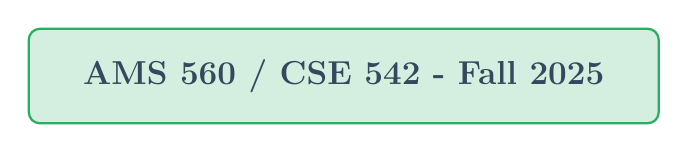
\begin{tikzpicture}
        \draw[accentgreen, thick, rounded corners, fill=accentgreen!20] (-4,-0.6) rectangle (4,0.6);
        \node[darkgray, font=\large\bfseries] at (0,0) {AMS 560 / CSE 542 - Fall 2025};
    \end{tikzpicture}
    
    \vspace{0.5cm}
    {\color{darkgray}\textbf{Team Members:}} \\
    Ahmad Javadi Nezhad • Daniel Bazmandeh • Iliya Mirzaei • Nicholas Tardugno • Tamali Halder
    
    \vspace{0.3cm}
    {\color{darkgray}September 2025}
\end{center}

\vspace{0.5cm}

% Section 1: Background and Motivation
\section{\color{primaryblue}Background and Motivation}

\textbf{Concrete Application:} DataMender targets \textit{ride-sharing companies} processing 5-10GB daily trip datasets with inconsistent formatting, missing timestamps, and duplicate records. Current solutions like OpenRefine require manual rule creation, while Trifacta/Alteryx use predefined transformations without LLM integration.

\textbf{The Gap:} No existing tool combines \textbf{automated LLM-powered rule discovery} with \textbf{human validation workflows} for large-scale data quality management. Data scientists spend 60-80\% of their time on data cleaning, yet lack tools that can suggest context-aware cleaning rules for multi-gigabyte datasets.

\textbf{Recent Work (2024-2025):} Recent studies show LLMs can generate data transformation rules, but existing implementations lack: (1) Large-scale file handling, (2) Human-in-the-loop validation, (3) Domain-specific rule templates, and (4) Hallucination mitigation strategies.

% Section 2: Problem Statement and Importance  
\section{\color{primaryblue}Problem Statement and Importance}

\textbf{Core Problem:} Organizations struggle to efficiently clean large CSV/Parquet files due to lack of automated rule discovery systems that can handle multi-gigabyte datasets.

\textbf{Why This Matters:} Data cleaning consumes 60-80\% of data science workflows, manual rule creation doesn't scale to large datasets, existing tools lack LLM integration, and poor data quality leads to unreliable analytics and ML models.

\textbf{Target Use Case:} Ride-sharing companies with 5-10GB CSV files containing millions of records with inconsistent formatting, missing values, and data quality issues requiring cleaning rules.

% Section 3: Challenges and Novelty
\section{\color{primaryblue}Challenges and Novelty}

\textbf{Technical Challenges:} Profiling multi-gigabyte files without memory overflow, designing effective LLM prompts, creating intuitive validation UI, ensuring vectorized operations for large-scale transformations.

\textbf{LLM Hallucination Mitigation:} (1) \textbf{Confidence Scoring:} Each suggested rule includes confidence metrics based on data coverage and pattern consistency, (2) \textbf{Multi-Model Validation:} Cross-validate rules using GPT-4, Claude-3, and local models, (3) \textbf{Human Validation Required:} All rules must pass human review before application, (4) \textbf{Reversible Operations:} All transformations are logged for easy rollback, (5) \textbf{Test Data Validation:} Rules tested on sample data before full application.

\textbf{Novel Contributions:} (1) First LLM-powered rule discovery for large-scale CSV/Parquet files, (2) Human-in-the-loop validation workflow, (3) Domain-specific templates for ride-sharing data, (4) Hallucination-resistant rule generation pipeline.

% Section 4: Solution Approach and Competitors
\section{\color{primaryblue}Solution Approach and Competitors}

\textbf{DataMender Components:} (1) \textbf{Data Profiler:} Fast scanning using Pandas/NumPy/Dask, (2) \textbf{LLM Rule Discovery Engine:} Multi-model prompts (GPT-4, Claude-3) with confidence scoring, (3) \textbf{Human Validation:} Interactive UI for reviewing/editing rules.

\textbf{Key Competitors:} OpenRefine (manual rules, no LLM), Trifacta/Alteryx (expensive, rule-based only), HoloClean (anomaly detection only, no rule generation).

\textbf{DataMender's Competitive Advantages:} (1) \textbf{First LLM-powered rule discovery} for large-scale data, (2) \textbf{Human-in-the-loop validation} preventing hallucinations, (3) \textbf{Domain-specific templates} for ride-sharing data, (4) \textbf{Multi-model validation} reducing false positives, (5) \textbf{Free and open-source} unlike enterprise tools.


% Section 5: Deliverables and Work Division
\section{\color{primaryblue}Deliverables and Work Division}

\textbf{8-Week Timeline:} Weeks 1-2: Dataset selection and profiler. Weeks 3-4: LLM prompts and UI tool. Weeks 5-6: Batch processing engine. Weeks 7-8: Testing and documentation.

\textbf{Final Deliverables:} (1) Working UI tool, (2) YAML configuration files, (3) Demo video, (4) Technical report with performance metrics vs. GPT-4, OpenRefine, Trifacta baselines.

\textbf{Work Division:} \textbf{Ahmad:} Project coordination, LLM integration, rule discovery engine development. \textbf{Daniel:} Data profiler implementation and optimization. \textbf{Iliya:} Validation UI design and interface development. \textbf{Nicholas:} Batch processing engine and data transformation. \textbf{Tamali:} Testing, metrics collection, documentation, and final report preparation.

All members will contribute to dataset selection, testing, and final presentation preparation.

\textbf{Expected Impact:} DataMender demonstrates LLM-powered rule discovery for large-scale data cleaning workflows, providing foundation for future AI-assisted data quality research.

\end{document}
